\label{cap:tests}
Wie im vorherigen Kapitel beschrieben, existieren verschiedene Varianten, einen \gc{} Tausch 
durchzuführen. Für das Finden der gemeinsamen Nachbarschaft betrachten wir sieben verschiedene Methoden, 
für das Tauschen der Nachbarschaft zwei. Weiterhin prüfen wir, ob es sinnvoll ist, 
die Variante der Vorsortierung zu nutzen oder nicht.
Kombiniert man all diese Möglichkeiten erhält man somit insgesamt 28 verschiedene Varianten einen \gc{} 
Tausch umzusetzen.
In diesem Kapitel diskutieren wir, welche der Varianten am geeignetsten ist.
%%%%%%%%%%%%%%%%%%%%%%%%%%%%%%%%%%%%%%%%%%%%%%%%%%%%%%%%%%%%%%%%%%%%%%%%
%%%%%% Aufbau
%%%%%%%%%%%%%%%%%%%%%%%%%%%%%%%%%%%%%%%%%%%%%%%%%%%%%%%%%%%%%%%%%%%%%%%%

\section{Versuchsaufbau}
Um die einzelnen Varianten auf ihre Laufzeit zu testen, wird ein Versuch aufgebaut.
Dazu werden alle Methoden in \cpp programmiert. Diese werden dann auf unterschiedlichen
Instanzen getestet und mittels Google Benchmark \cite{benchmark} wird die Zeit gemessen, 
die für das Ausführen benötigt wurde.
\\

Wie beschrieben benötigen die Methoden als Eingabe keinen Graph, 
sondern lediglich zwei Arrays, welche jeweils die Nachbarschaft zweier Knoten repräsentieren. Ohne 
Beschränkung der Allgemeinheit nennen wir das größere Array \fett{large}, das kleinere \fett{small}.
Um möglichst gut zu erkennen, wie sich die verschiedenen Methoden bei unterschiedlichen
Eingaben verhalten, messen wir die Laufzeiten für eine ganze Reihe an Instanzen. 
Um ein gutes Bild zu erhalten, sollten folgende Fälle abgedeckt sein:

\begin{itemize}
	\item Beide Arrays liegen in der gleichen Größenordnung
	
	\item Eines der Arrays ist wesentlich größer als das andere
	
	\item Der Anteil an gemeinsamen Elementen ist groß
	
	\item Der Anteil an gemeinsame Elementen  ist klein
\end{itemize}

Um dies zu erreichen, wird jedes Experiment in  mehreren Runden durchgeführt, in denen das Array large von anfänglich 128
Elementen auf bis zu 4.000.000 Elementen vergrößert wird. 
Jede Runde besteht aus mehreren Durchläufen, bei denen das Array small eine Größe zwischen 32 Elementen und der jeweiligen Größe von large hat.
Für jeden dieser Durchläufe werden die beiden Arrays mit zufälligen, aber paarweise verschiedenen
Werten befüllt, bis sie die entsprechende Größe haben. 
Dabei existiert jedoch kein Element, welches in beiden Arrays 
enthalten ist, was dazu führen würde, dass ein \gc{} 
Tausch nichts verändern würde. Um sicherzugehen,
dass die gemeinsame Nachbarschaft nicht leer ist, müssen somit Elemente des einen Arrays 
in das andere hineinkopiert werden. Damit die Größe der gemeinsamen Nachbarschaft
variiert wird, werden zuerst 10, dann 25, 50 und 75 Prozent der Elemente kopiert. 
\\

Eine einzelne Test-Messung lässt sich somit durch ein Tripel \fett{(\la, \sm, \fr)} beschreiben, wobei
large  und small für die Größe der jeweiligen Arrays stehen.
Der Wert \fett{\fr} steht dabei für den prozentualen Anteil der gemeinsamen Elemente an small.





%%%%%%%%%%%%%%%%%%%%%%%%%%%%%%%%%%%%%%%%%%%%%%%%%%%%%%%%%%%%%%%%%%%%%%%%
%%%%%% Messung
%%%%%%%%%%%%%%%%%%%%%%%%%%%%%%%%%%%%%%%%%%%%%%%%%%%%%%%%%%%%%%%%%%%%%%%%

\section{Messung}
\label{sec:messung}
Auf die im vorherigen Abschnitt beschriebene Weise werden die verschiedenen Instanzen erstellt und
mittels Google Benchmark die Zeit gemessen. Aus Zeitgründen werden jedoch nicht alle Werte 
für \la{} und \sm{} erstellt. Deshalb verdoppeln wir in jedem Schritt die Werte von \la{} und \sm{,}
anstatt sie um eins zu inkrementieren. Somit ergeben sich insgesamt 672 Instanzen, auf denen die Laufzeiten der 
einzelnen Methoden gemessen werden. 
Um Rauschen zu verringern, wird dabei jede Variante so oft wiederholt
 bis mindestens 100ms gemessen wurden.
Um eventuelle Messfehler zu minimieren, wird
dieser Vorgang jeweils fünf mal wiederholt. 
Als resultierender Messwert dient der Mittelwert dieser Wiederholungen.
\\

Alle Messungen wurden auf einem Rechner mit 64GB Arbeitsspeicher und einem Prozessor vom Typ Intel(R) Xeon(R) CPU E5-2630 v3 @ 2.40GHz,
mit 8 Kernen, Hyperthreading und einem Cache von 20 MB, ausgeführt.
Mit dieser Konfiguration hat die Dauer für alle 28 Varianten in Summe ungefähr 19 Stunden betragen.




%%%%%%%%%%%%%%%%%%%%%%%%%%%%%%%%%%%%%%%%%%%%%%%%%%%%%%%%%%%%%%%%%%%%%%%%
%%%%%% Auswertung
%%%%%%%%%%%%%%%%%%%%%%%%%%%%%%%%%%%%%%%%%%%%%%%%%%%%%%%%%%%%%%%%%%%%%%%%

\section{Auswertung}
\label{ref:auswertung}
Die ermittelten Messdaten werden schließlich mit Hilfe von 
Jupyter Notebook \cite{jupyter} ausgewertet. Dabei
handelt es sich um ein Tool, mit dem man Python-Programme auf einfache Art und Weise erstellen und 
ausführen kann.
Innerhalb von Python nutzen wir die Bibliotheken \fett{Matplotlib} und \fett{pandas}, um die Daten
zu analysieren und grafisch aufzuarbeiten.
\begin{figure}
\centering
	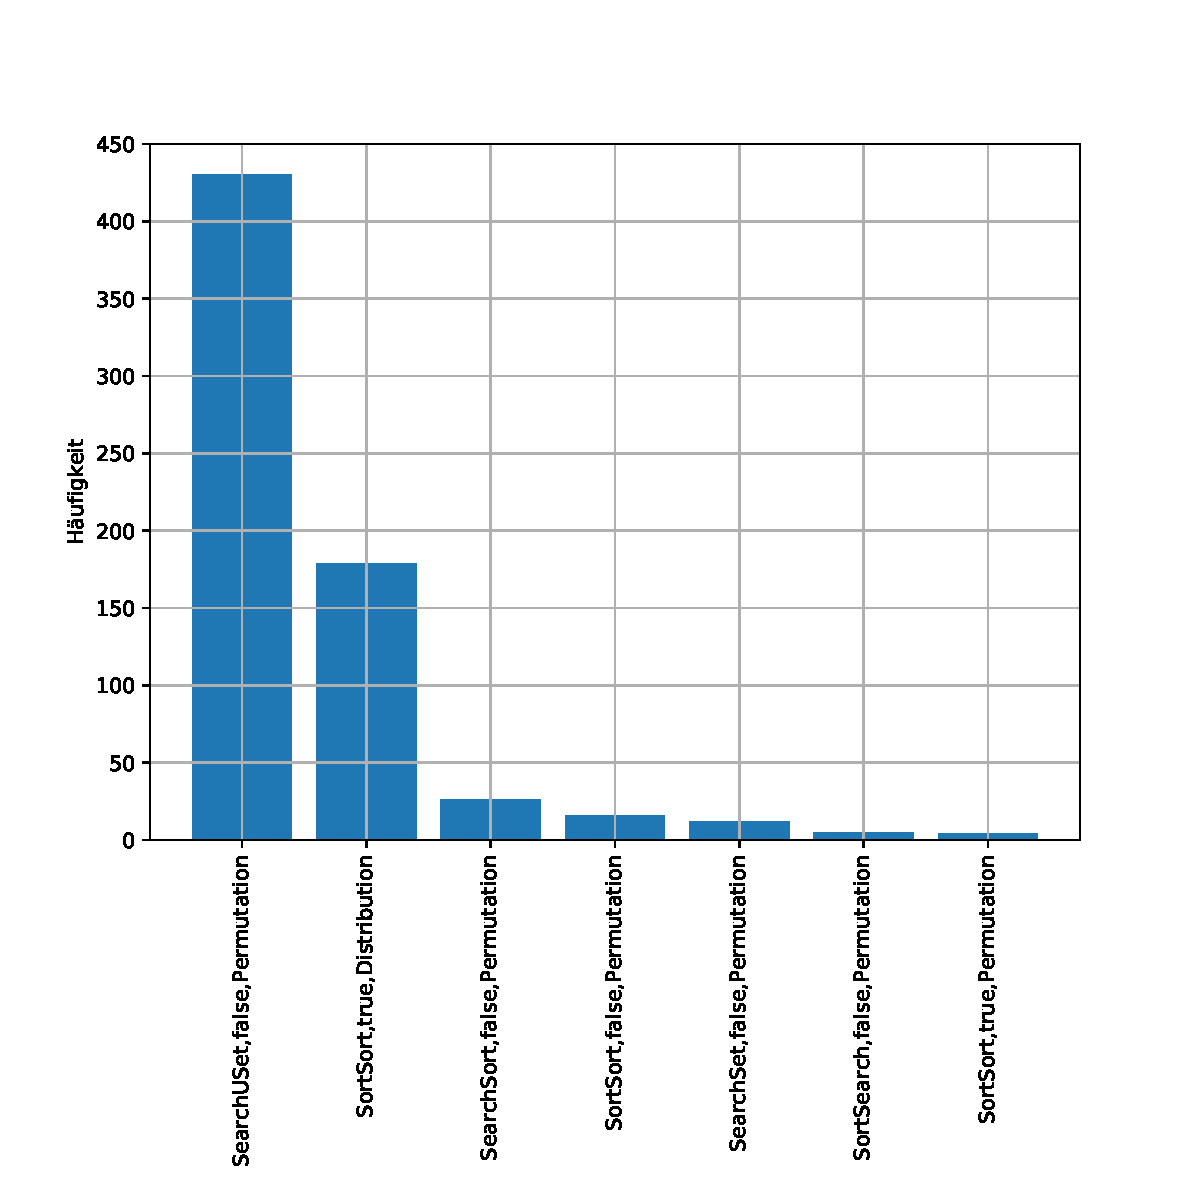
\includegraphics[width = 0.65\textwidth]{figures/counting.pdf}
	\caption{Vergleich der Varianten, welche am häufigsten die geringste Laufzeit aufweisen}
	\label{fig:messung_counting}
\end{figure}
\\

Zuerst betrachten wir für jede Instanz, welche Methode am schnellsten war.
Interessant sind dann jeweils die Methoden, für die häufig die geringste Laufzeit gemessen wurde.
In Abbildung \ref{fig:messung_counting} ist dazu ein Balkendiagramm dargestellt.
Dabei sieht man eindeutig, dass die Variante (\SeaUSet, \false, \perm) mit Abstand 
auf den meisten Instanzen die schnellste Laufzeit aller Methoden hat. Die
430 Instanzen auf welchen (\SeaUSet, \false, \perm) die schnellste Methode ist, entsprechen einem Anteil von rund
64\%. Mit 179 \glqq gewonnenen\grqq{} Instanzen folgt die Variante (\SorSor, \true, \distr), was einem Anteil von
27\% entspricht. Zusammen ist somit in etwa 91\% aller getesteter Instanzen eine dieser beiden Methoden
die Schnellste gewesen. Daher liegt der Schluss nahe, sich beim Suchen der \glqq besten\grqq{} Variante,
auf diese beiden Methoden zu beschränken. 
\\

Um nicht fälschlicherweise \glqq gute\grqq{} Methoden auszuschließen,
betrachten wir einen weiteren Plot in Abbildung \ref{fig:messung_slowdown}. 
\begin{figure}
\centering
	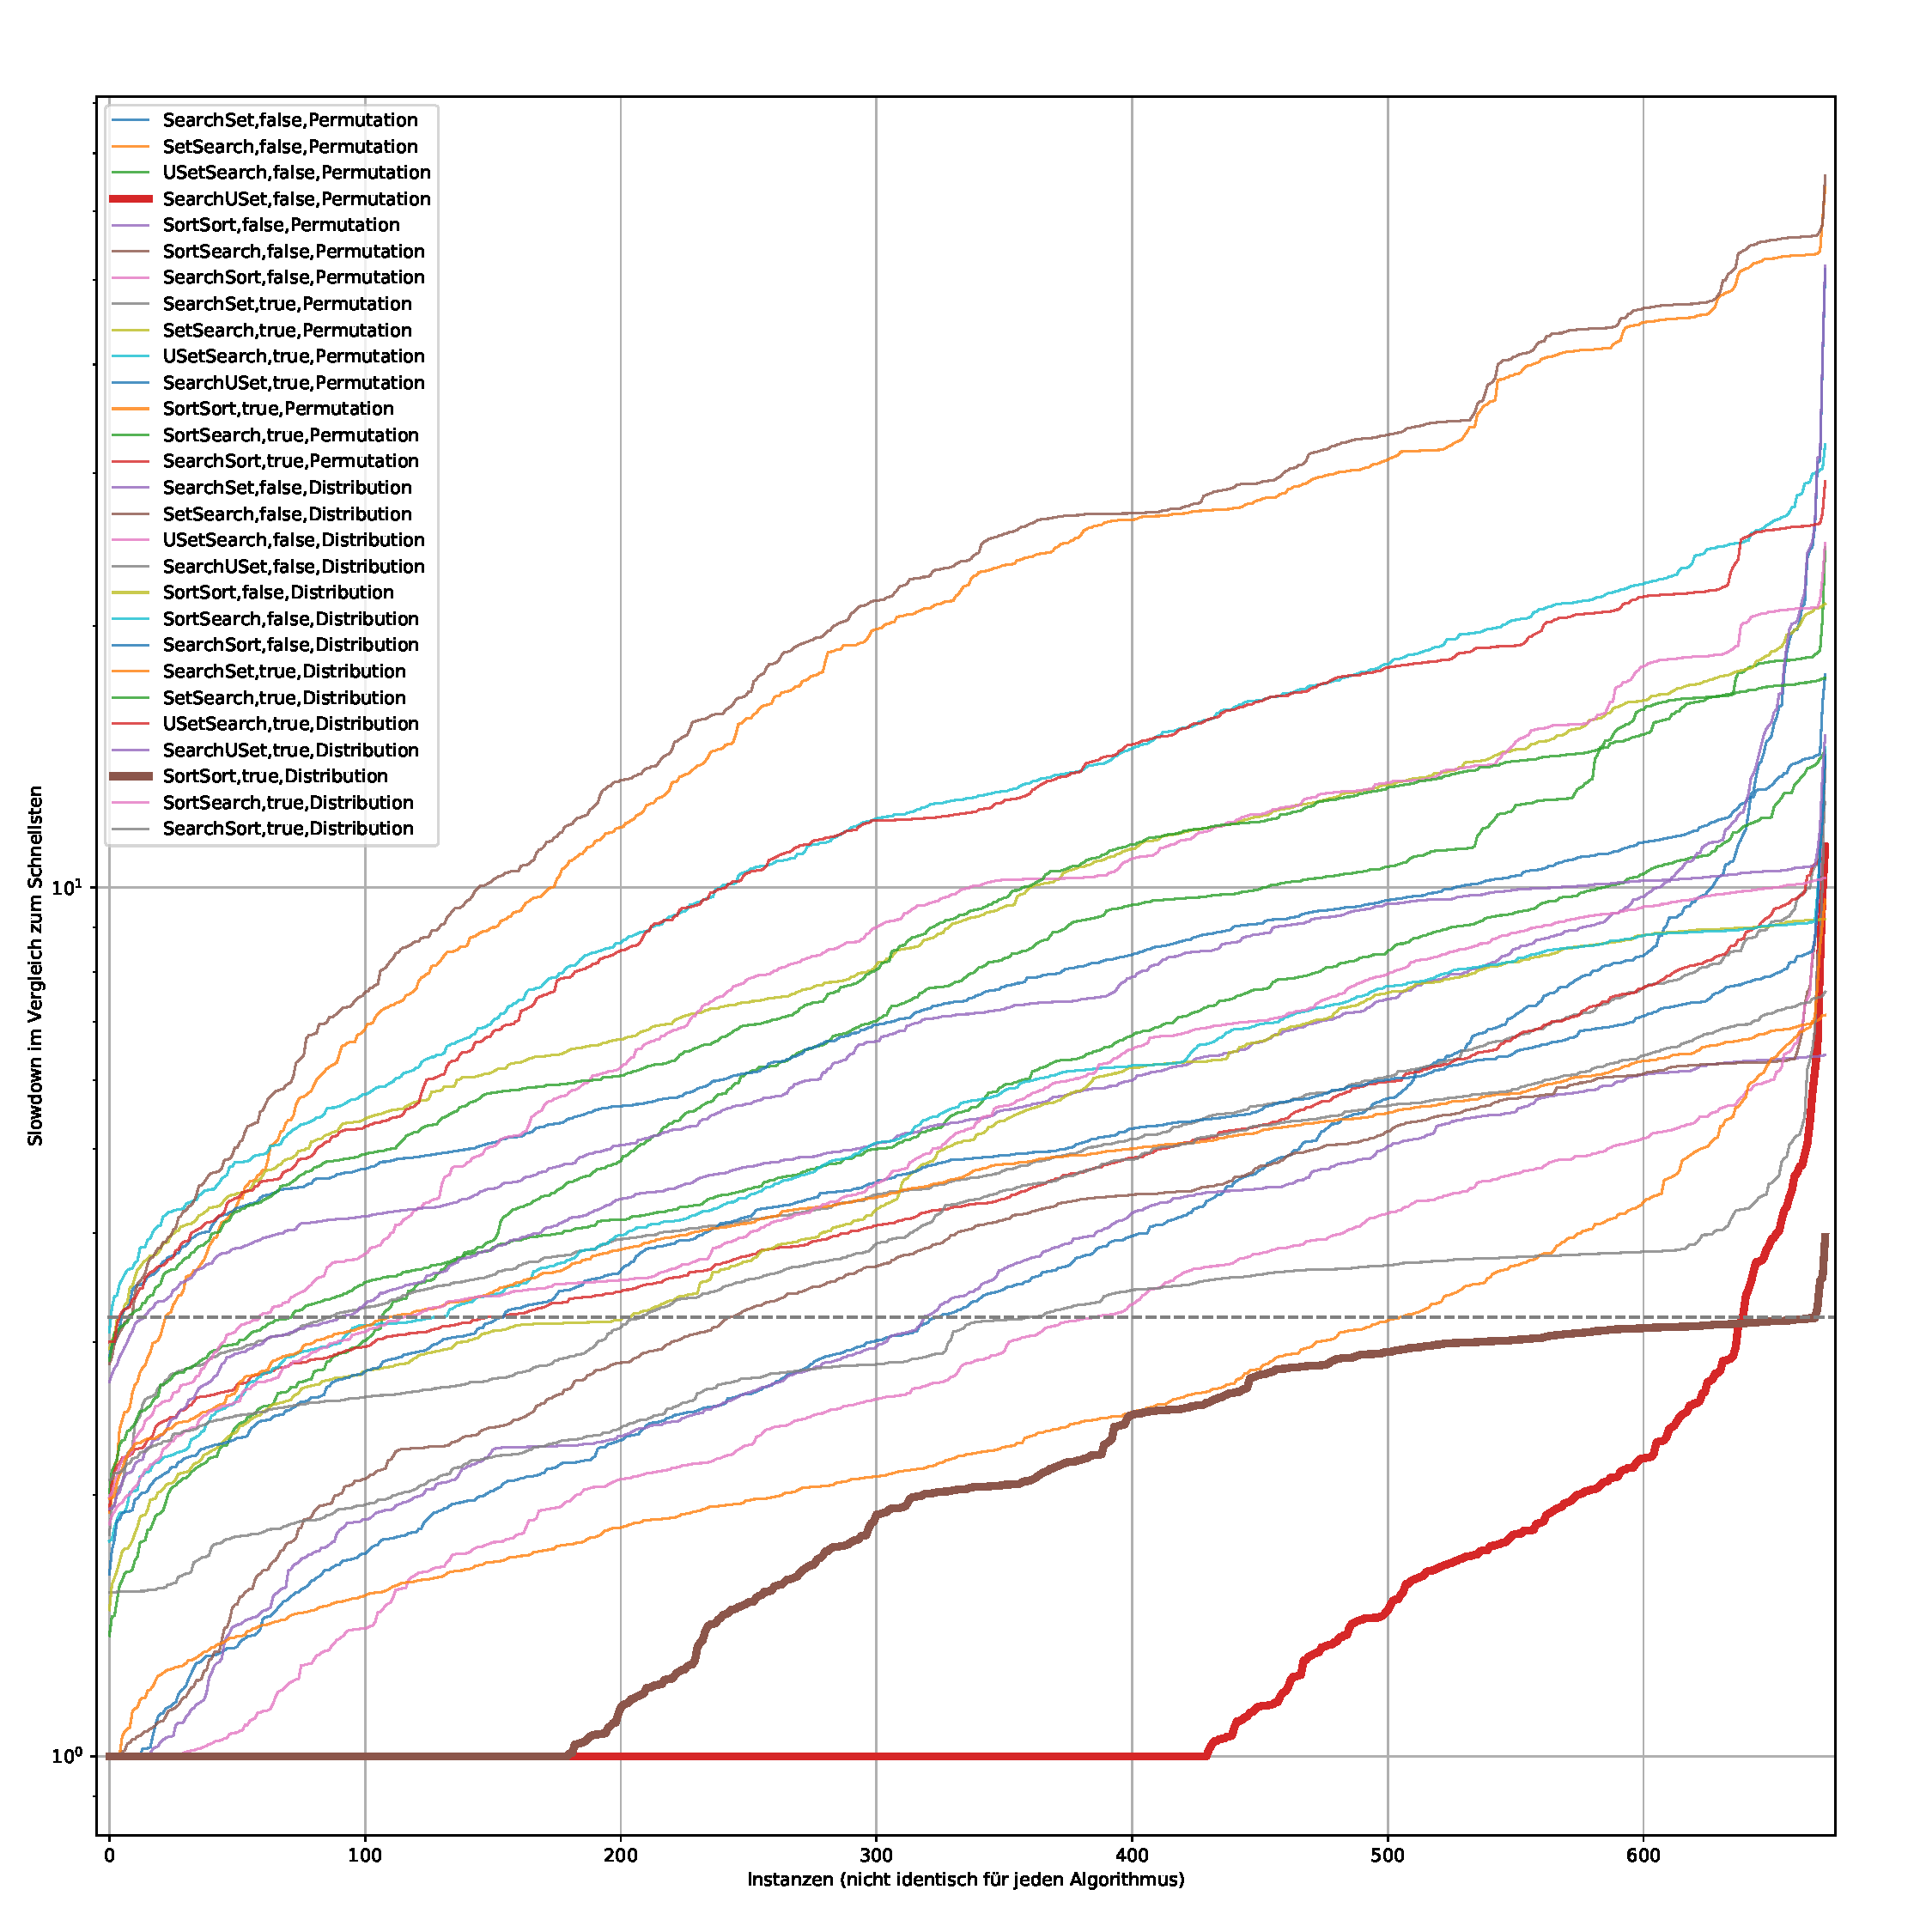
\includegraphics[width = 1\textwidth]{figures/slowdown.pdf}
	\caption[Slowdown der einzelnen Varianten im jeweiligen Vergleich zur Variante mit der geringsten Laufzeit.]
	{Slowdown der einzelnen Varianten im jeweiligen Vergleich zur Variante mit der geringsten Laufzeit. 
	Dabei ist der Wert 3.5 als gestrichelte Linie eingezeichnet}
	\label{fig:messung_slowdown}
\end{figure}
Um diesen Plot zu erstellen, wurde jede Variante einzeln betrachtet.
Dann wird für jede Instanz bestimmt, welche Variante die kürzeste Laufzeit hat und der Quotient
aus dieser Laufzeit und der Laufzeit der betrachteten Variante berechnet. Dieses Verhältnis wird als Slowdown
bezeichnet und gibt an, um welchen Faktor die Variante langsamer als die schnellste ist. Die Slowdowns
zu jeder Instanz werden schließlich aufsteigend sortiert und als Kurve in den Plot eingefügt.
Da die Slowdowns jedoch für jede Variante unabhängig voneinander sortiert werden, geht dadurch 
die Ordnung über die Instanzen verloren. Somit entspricht eine Stelle auf der horizontalen Achse 
nicht für jede Variante der gleichen Instanz. Einen \glqq guten\grqq{} Algorithmus erkennt man in diesem
Plot, wenn die entsprechende Kurve lange nahe der eins verläuft.
\\

Dieser Plot legt ebenfalls nahe, sich auf die beiden Varianten (\SeaUSet, \false, \perm) und 
(\SorSor, \true, \distr) zu konzentrieren, da die beiden Kurven am wenigsten stark wachsen und damit 
die Slowdowns vergleichsweise klein sind. Jedoch lässt sich auch hier nicht bestimmen, welche der beiden
Varianten die bessere ist. Ein Vorteil von (\SeaUSet, \false, \perm) ist, 
dass die Methode auf den meisten Instanzen einen Slowdown
von eins hat ---was wir ja auch schon in Abbildung \ref{fig:messung_counting} gesehen haben---
und damit langsamer anwächst. Ein Nachteil liegt aber darin, dass der Slowdown für manche Instanzen
eine Größe von bis zu 10 erreicht, während der Slowdown von  (\SorSor, \true, \distr) durch den maximalen
Wert von 3.5 beschränkt ist.
\newpage
Dieser Nachteil spiegelt sich ebenfalls in Abbildung \ref{fig:messung_mean} wieder. Für diesen Plot
wurde über alle Instanzen für jede Variante jeweils die mittlere Laufzeit bestimmt. Obwohl
es nicht in den meisten Fällen die schnellste Variante ist, hat (\SorSor, \true, \distr) die 
kleinste mittlere Laufzeit mit rund 38 Millisekunden. Auf Platz zwei folgt
(\SeaUSet, \false, \perm) mit etwa 64 Millisekunden, was schon einer Abweichung von ungefähr 60\% entspricht.
Auch in diesem Plot sieht man deutlich, dass es sich nicht lohnt, noch weitere Varianten zu betrachten. Zwar hat 
auch (\SorSor, \true, \perm) eine mittlere Laufzeit, 
die annähernd so groß ist wie die Laufzeit von (\SeaUSet, \false, \perm), aber 
auch diese kommt nicht an die Schnellste heran. Alle anderen Varianten 
haben eine deutlich größere mittlere Laufzeit.
\begin{figure}
\centering
	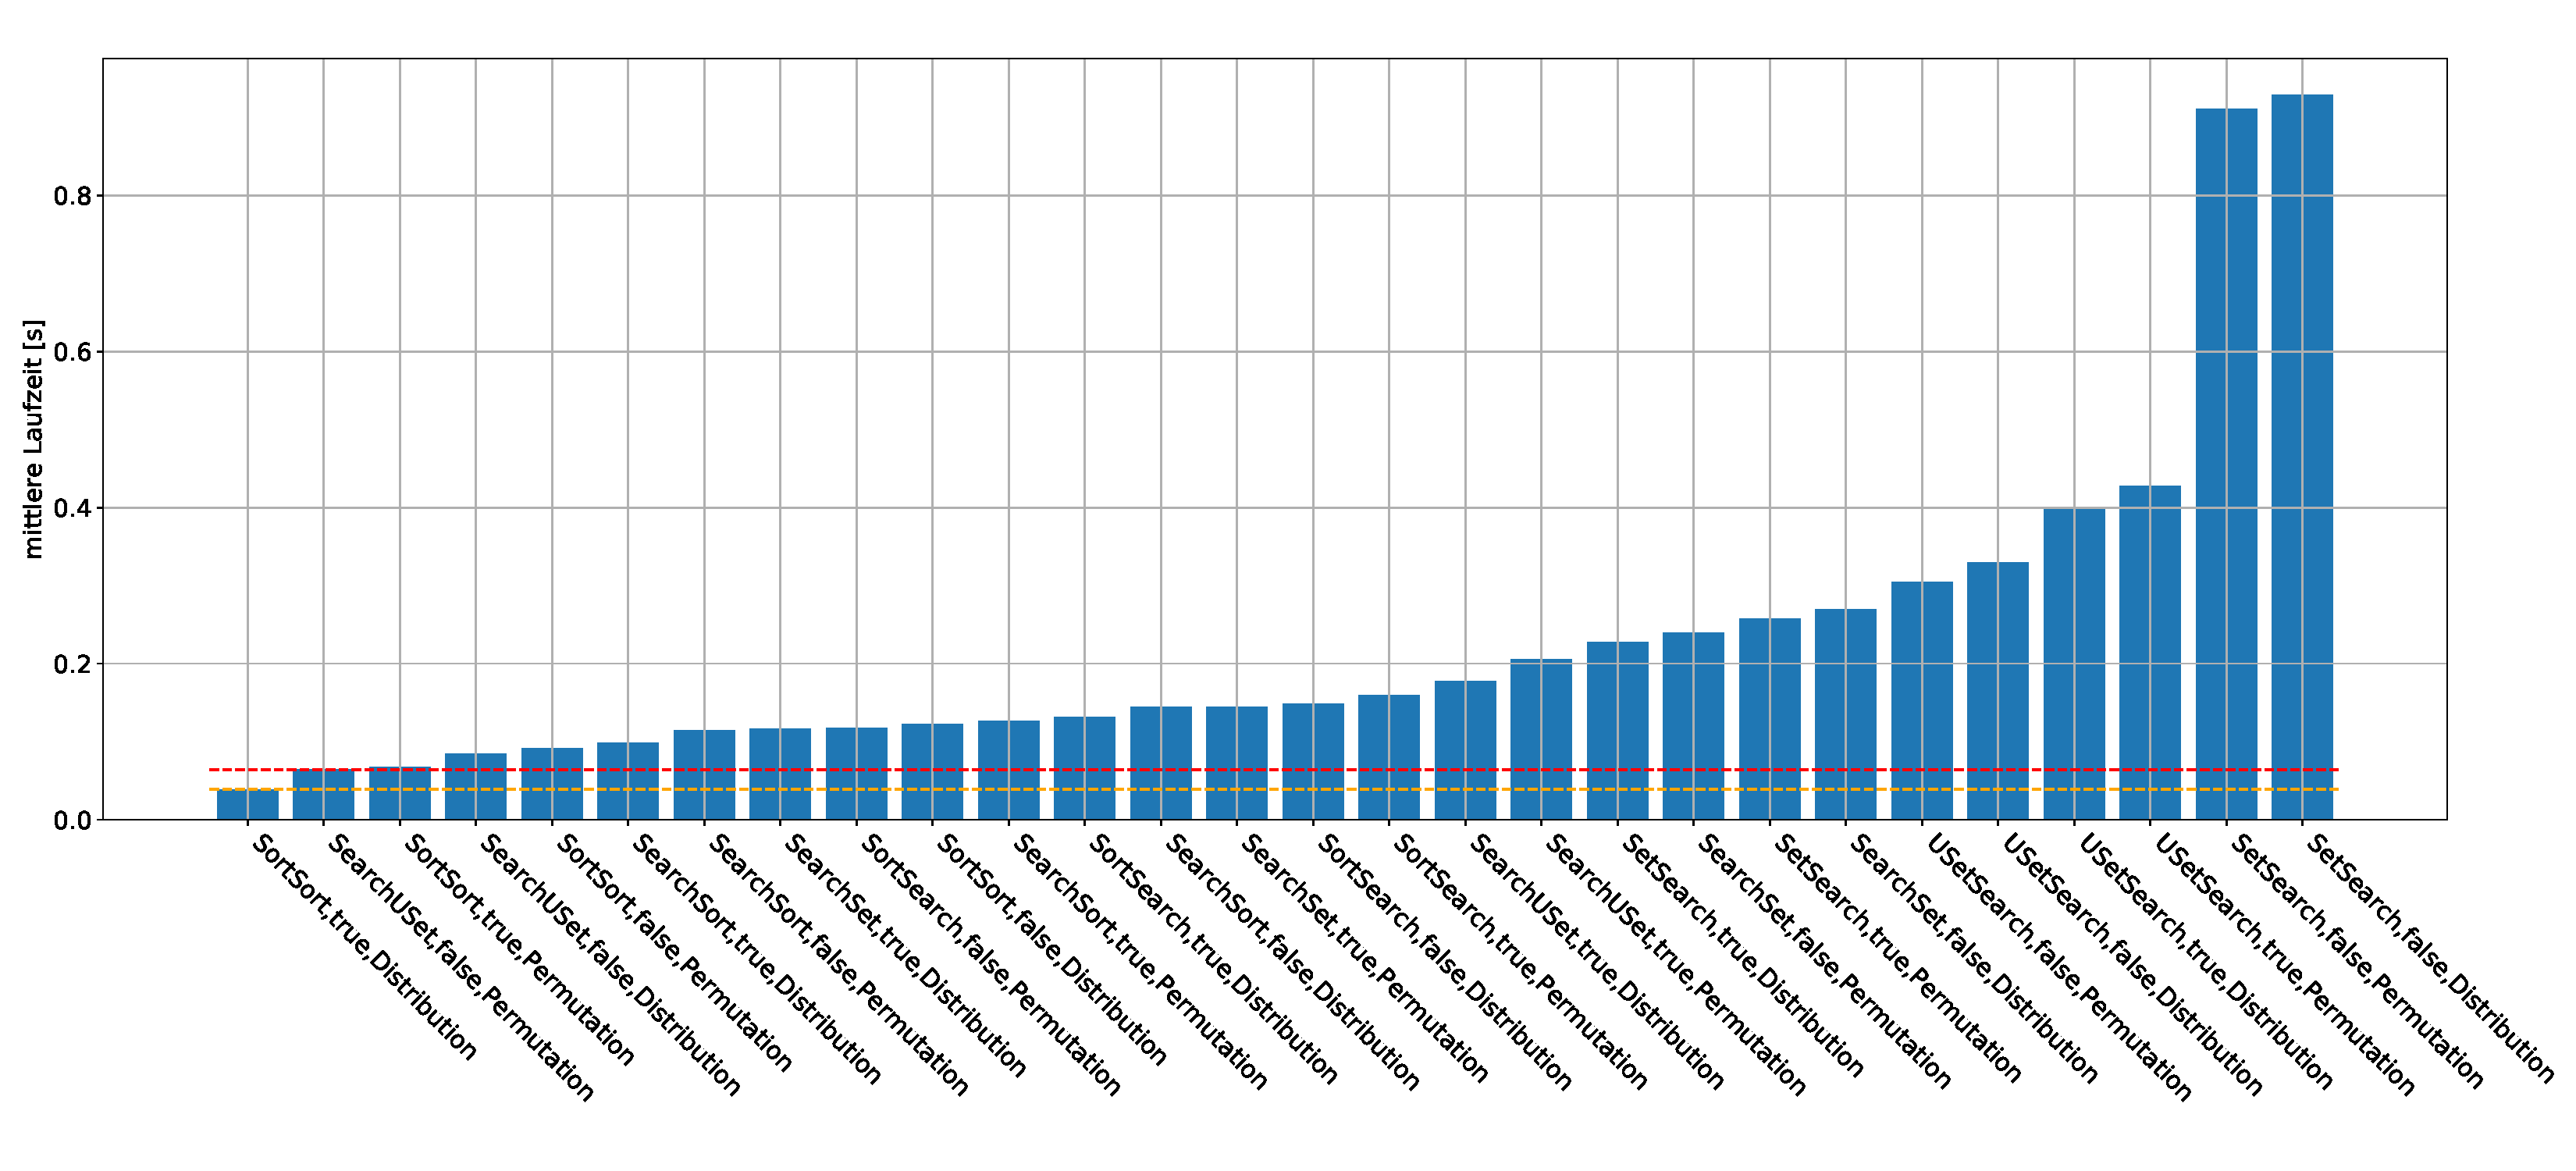
\includegraphics[width = \textwidth]{figures/mean.pdf}
	\caption{Mittlere Laufzeiten der Varianten über allen Instanzen}
	\label{fig:messung_mean}
\end{figure}
\\

Abschließend betrachten wir noch die zwei ausgewählten Varianten im direkten Vergleich. Hierzu wurden
in Abbildung \ref{fig:messung_small} auf der horizontalen Achse die getesteten Instanzen aufgetragen
und dazu die jeweiligen Laufzeiten von (\SorSor, \true, \distr) und (\SeaUSet, \false, \perm) als Punkte
eingezeichnet. 
Man sieht dabei, dass sich die Laufzeiten in den meisten Instanzen nicht so stark unterscheiden.
Dies sind vor allem die Instanzen, bei denen der Unterschied zwischen \la{} und \sm{} nicht so groß ist.
In den Instanzen, in denen sich die Werte für \sm{} und \la{} stark unterscheiden, ist jedoch ein 
deutlicher Vorteil von (\SorSor, \true, \distr) zu erkennen. Auch bei den \glqq großen\grqq{} Instanzen
mit Werten von $\text{\sm{}}> 500.000$ hat diese Variante einen deutlichen Laufzeitvorteil.
Auf der Instanz (4.194.304, 4.194.304, 75) beispielsweise hat (\SeaUSet, \false, \perm) eine Laufzeit
von circa 1,628 Sekunden, während (\SorSor, \true, \distr) nur etwa 0,146 Sekunden benötigt. Der Slowdown
beträgt für diese Instanz also in etwa einem Wert von 11. 
\begin{figure}
\centering
	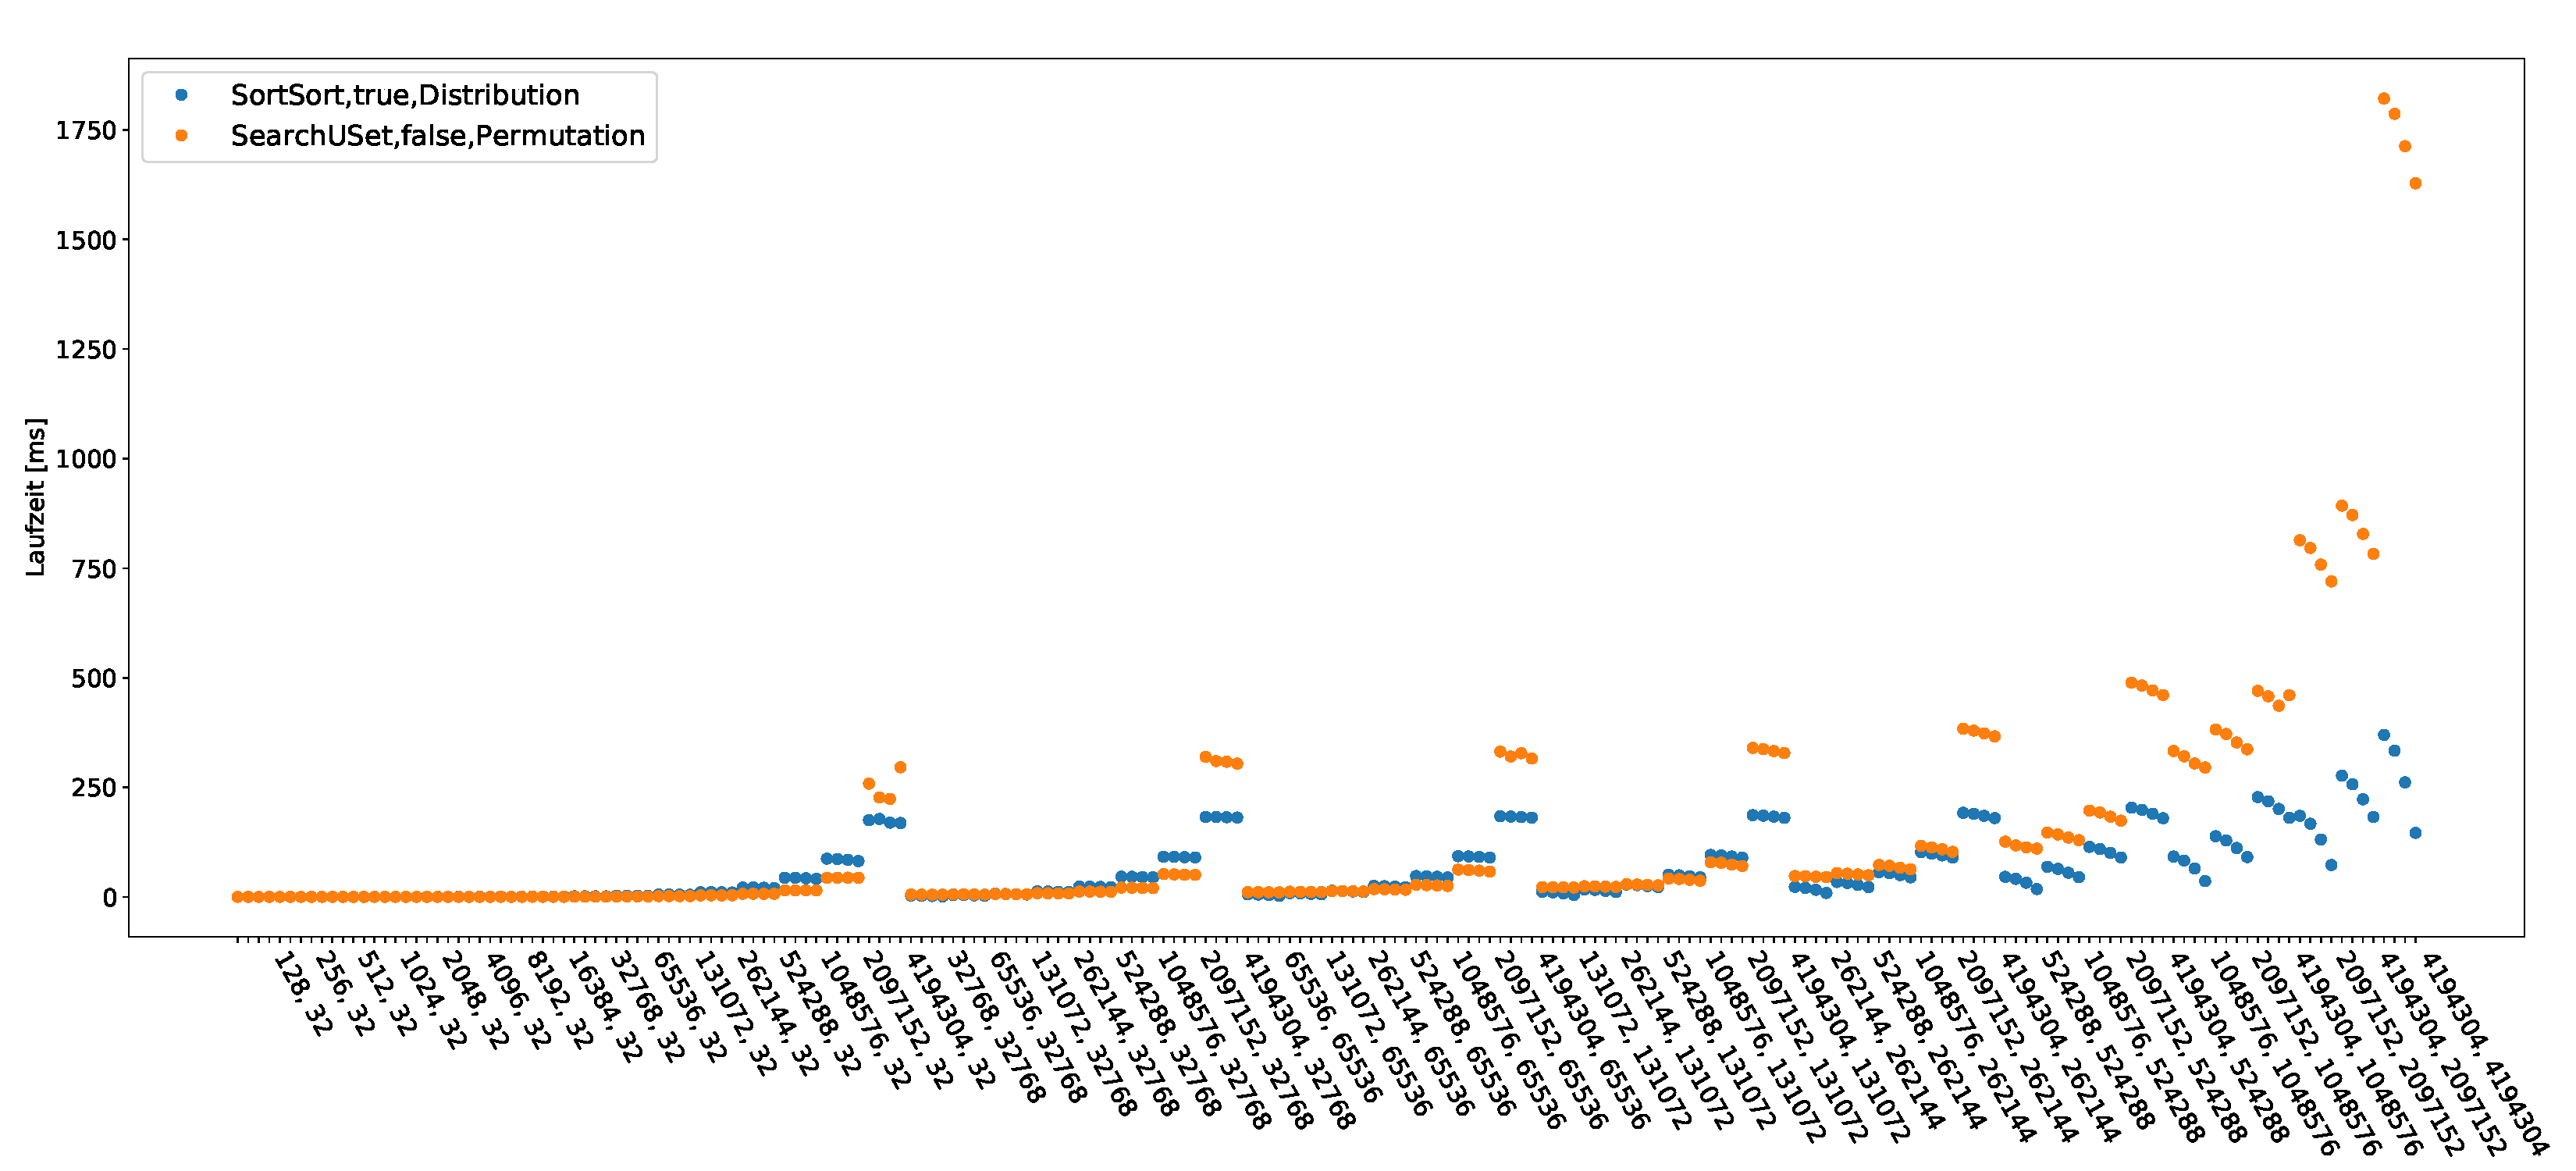
\includegraphics[width = \textwidth]{figures/small_aufsteigend.pdf}
	\caption[Laufzeitvergleich der zwei besten Varianten auf ausgewählten Instanzen] {Vergleich der Laufzeiten der zwei besten Varianten auf ausgewählten Instanzen.
			Die Instanzen sind nach aufsteigenden Werten für \sm{} sortiert. Aus Gründen der Übersichtlichkeit
wird bei  der Beschriftung der Instanzen der Teil \fr{} weggelassen, die Instanzen werden 
nur mit \la{}, \sm{} bezeichnet. Weiterhin wurden der
Übersichtlichkeit wegen die Instanzen aus dem Bereich $32 < \text{\sm}  <32768$ ausgelassen, da sie das gleiche
Bild wie die üblichen Instanzen zeigen.}
	\label{fig:messung_small}
\end{figure}

%%%%%%%%%%%%%%%%%%%%%%%%%%%%%%%%%%%%%%%%%%%%%%%%%%%%%%%%%%%%%%%%%%%%%%%%
%%%%%% Diskussion
%%%%%%%%%%%%%%%%%%%%%%%%%%%%%%%%%%%%%%%%%%%%%%%%%%%%%%%%%%%%%%%%%%%%%%%%

\section{Diskussion der Ergebnisse}
Es gilt zu überprüfen, ob die ermittelten Ergebnisse zu erwarten waren, indem wir sie 
mit den asymptotischen Laufzeiten aus der Tabelle \ref{tab:varianten} vergleichen.
Laut den asymptotischen Laufzeiten sollte die Variante mit \SorSor{}, \distr{} und vorsortiert am schnellsten
sein. Dies sieht man auch bei den mittleren gemessenen Laufzeiten aus Abbildung \ref{fig:messung_mean}.
Dabei liegt diese Variante deutlich auf dem ersten Platz. Die dazugehörige Variante mit
der Tausch-Methode \perm{} liegt auf dem dritten Platz, obwohl sie im Vergleich eine der
schlechtesten asymptotischen Laufzeiten hat. Der Grund für diese Diskrepanz 
liegt vermutlich darin, dass diese
asymptotische Laufzeit durch das einmalige Sortieren am Ende der Methode entsteht. 
In anderen Varianten, welche die gleiche asymptotische Laufzeit haben, wird jedoch eventuell häufiger
sortiert oder eine Datenstruktur verwendet, die eine höhere Laufzeit produziert.
\\

Auffällig ist, dass die Varianten mit \USetSea{} jeweils deutlich langsamer sind als die analogen
Varianten, welche \SeaUSet{} verwenden, obwohl die erwarteten asymptotischen Laufzeiten
gleich sind. Dies liegt höchstwahrscheinlich an der
Datenstruktur \texttt{unordered\_set}, einer Hash-Tabelle. Bei dieser Datenstruktur
sind die Laufzeiten stark abhängig vom Füllgrad, also dem Anteil der 
gespeicherten Elemente im Bezug zur Größe der Hash-Tabelle. Da bei \USetSea{} die Elemente
des größeren Arrays in die Hash-Tabelle eingefügt werden, ist der Füllgrad dementsprechend
auch größer, was zu der schlechteren Laufzeit führt.
Im Gegensatz dazu ist die Methode, welche \SeaUSet, \perm{} und keine Vorsortierung verwendet,
die im Mittel zweitschnellste aller gemessenen Varianten, da sich hierbei
weniger Elemente in der Hash-Tabelle befinden und der Füllgrad demnach geringer ist. 
Somit wird auch eher die Laufzeit des Erwartungswerts erreicht.
\\

Mit einem ähnlichen Argument lassen sich auch die schlechten Laufzeiten 
der Varianten, welche \SetSea{} verwenden, erklären. Hierbei wird ebenfalls das größere
Array in die Datenstruktur eingefügt, was zu der schlechteren Laufzeit führt.  
Dabei fällt jedoch noch auf, dass vor allem die Varianten, 
bei welchen nicht vorsortiert wird, die mit Abstand längsten Laufzeiten besitzen. Als Begründung 
dient hier, dass beim Erstellen des Binärbaums für jeden Knoten, welcher eingefügt wird,
eine Speicherallokation ausgeführt wird, was sehr laufzeitintensiv ist. Ist die
Eingabe bereits sortiert, kann dies von der Implementierung des Binärbaums ausgenutzt werden.
\\

Insgesamt wirken die gemessenen mittleren Laufzeiten 
also plausibel.



%%%%%%%%%%%%%%%%%%%%%%%%%%%%%%%%%%%%%%%%%%%%%%%%%%%%%%%%%%%%%%%%%%%%%%%%
%%%%%% Fazit
%%%%%%%%%%%%%%%%%%%%%%%%%%%%%%%%%%%%%%%%%%%%%%%%%%%%%%%%%%%%%%%%%%%%%%%%

\section{Auswahl der besten Variante}
\label{sec:entscheidung}
Abschließend muss anhand der Messdaten entschieden werden, welche Variante zum Einsatz für
einen \ct{} am besten geeignet ist.
Zusammenfassend haben wir im Abschnitt \ref{ref:auswertung} festgestellt, 
dass hierfür nur die Varianten (\SorSor, \true, \distr) und (\SeaUSet, \false, \perm) zur Auswahl stehen.
Während die eine Variante am häufigsten die geringste Laufzeit hat, liegt die andere 
bei der durchschnittlichen Laufzeit weiter vorne. Dies liegt vor allem daran, dass sich 
die Laufzeiten bei den Instanzen, auf denen (\SeaUSet, \false, \perm) \glqq gewinnt\grqq{}, kaum unterscheiden.
Unter den anderen Instanzen gibt es jedoch welche, bei denen (\SorSor, \true, \distr) bis auf einen
Faktor von circa 11 schneller ist.
\\

Um ein bestmögliches Laufzeitverhalten für einen \ct{} zu erreichen, könnte man auf die Idee kommen, 
beide Varianten zusammen zu nutzen
und dabei eine Heuristik entwickeln, die jeweils angibt,
auf welcher Instanz man welche Variante verwenden sollte. Somit würde bei jedem \ct{} abhängig von 
der Eingabe, also den Nachbarschaften, entschieden werden, welche der beiden Instanzen man benutzt. 
Das Problem dabei liegt jedoch darin, dass bei diesen Varianten einmal die Vorsortierung
genutzt wird und einmal nicht. Dies ist allerdings nicht beides gemeinsam möglich. Entweder hält man die
Nachbarschaften immer sortiert, oder nicht. Man muss sich also für eine Möglichkeit dieser
Variante  entscheiden. Dadurch ändert sich dann aber zwangsläufig  eine der beiden anderen Varianten. 
Entscheidet man sich die Nachbarschaften sortiert zu halten, würde (\SeaUSet, \false, \perm) zu (\SeaUSet, \true, \perm){}
werden, andernfalls würde sich (\SorSor, \true, \distr) zu (\SorSor, \false, \distr) verändern.
Diese beiden \glqq veränderten\grqq{} Varianten haben aber jeweils deutlich schlechtere Laufzeiten
als die ursprünglichen.
\\

Es ist also nicht sinnvoll möglich, die beiden Varianten miteinander zu kombinieren. Wir müssen uns
also auf eine Variante festlegen. Dies ist die Variante (\SorSor, \true, \distr), da sie im Vergleich zur
Alternative ---wie schon beschrieben---
in kaum einer Instanz eine wesentlich schlechtere Laufzeit hatte, jedoch auf manchen Instanzen wesentlich
bessere Laufzeiten. Außerdem ist es die Variante mit der geringsten mittleren Laufzeit. 
Ein Vorteil dieser Variante neben der Laufzeit liegt noch in der Einfachheit. So werden
lediglich die beiden Arrays sortiert und linear durchlaufen. Es muss keine weitere Datenstruktur
erstellt werden ---wie bei der anderen Variante das \texttt{unordered\_set}--- und damit wird
auch kein zusätzlicher Speicherplatz verbraucht.


%%%%%%%%%%%%%%%%%%%%%%%%%%%%%%%%%%%%%%%%%%%%%%%%%%%%%%%%%%%%%%%%%%%%%%%%
%%%%%% Fazit
%%%%%%%%%%%%%%%%%%%%%%%%%%%%%%%%%%%%%%%%%%%%%%%%%%%%%%%%%%%%%%%%%%%%%%%%


\section{Vergleich zum Standard \cb{}}
\label{kap:result}
In einem letzten Experiment wird geprüft, wie sich die Laufzeit der bipartiten \gc{}
Variante, sowohl im parallelen als auch im sequenziellen Fall,
 im Vergleich zum \cb{} auf massiven Graphen verhält.
\\

Dazu werden wir verschiedene Test-Instanzen erstellen.
Als Grundlage dient ein Netflix-Datensatz\cite{kaggle}, welcher Nutzer- und Film-Knoten enthält, 
wobei eine gerichtete Kante von einem Film zu einem Nutzer gezogen wird, wenn dieser den 
Film gut bewertet hat. Damit liegen die Film-Knoten in einer Partitionsklasse und 
die Nutzer-Knoten in der anderen.
Aus diesem Graph werden drei Subgraphen erstellt, wobei jeweils 1000, 10.000 und 100.000  zufällige
Nutzer-Knoten ausgewählt werden und deren vollständige Nachbarschaft hinzugefügt wird.
Für jeden dieser drei Graphen gibt es zwei Varianten. Der Unterschied
zwischen den beiden Varianten liegt darin, welche der beiden Partitionsklassen aktiv sind, 
also auf welcher Partitionsklasse die \ct{e} ausgeführt werden.
Somit ergeben sich sechs Instanzen. 
\\

Auf diesen wird 
die in dieser Arbeit erarbeite bipartite Version des \gc{} ausgeführt. Dazu müssen die
einzelnen Graphen jedoch jeweils in einen ungerichteten Graph transformiert werden.
\\

Als Vergleich verwenden wir an dieser Stelle nicht 
den Standard \gc{} Algorithmus. Dies liegt daran, 
dass bei diesem Algorithmus auf bipartiten Graphen die Eigenschaft der
Bipartitheit verletzt werden könnte und zusätzlich viele unnötige \ct{e} ausgeführt werden. 
Auf einem bipartiten Graphen liegen in der disjunkten Nachbarschaft zweier Knoten, 
welche nicht aus der gleichen Partitionsklasse stammen, entweder keine Knoten,
 oder die beiden Knoten selbst. 
Führt man nun ein \ct{} auf diesen beiden Knoten aus, verändert sich entweder (im Falle einer leeren disjunkten
Nachbarschaft) nichts
oder es könnte passieren, dass ein Knoten sich selbst in seine Nachbarschaft getauscht bekommt.
Damit hätte dieser Knoten eine Kante zu sich selbst, was es jedoch auf bipartiten Graphen nicht 
geben darf.
\\

Deshalb wird als Vergleich der Standard \cb{} Algorithmus \cite{DBLP:conf/esa/CarstensH0PTW18}
sowohl auf den ungerichteten als auch auf den gerichteten Graphen ausgeführt.
Um die Probleme, welche wir für den \gc{} Algorithmus beschrieben haben, zu umgehen, 
führen wir die einzelnen \ct{e} ausschließlich auf Knoten einer Partitionsklasse aus.
\\

Um zusätzlich zu sehen, wie stark die Parallelisierung die Laufzeit des bipartiten
\gc{} beeinflusst, werden wir weiterhin eine sequenzielle Variante des bipartiten \gc{} 
untersuchen.
\\

Alle vier beschriebenen Varianten werden nacheinander auf dem gleichen Prozessor ausgeführt, welcher 8
Kerne mit Hyperthreading besitzt. Es werden bei jeder Variante insgesamt 10 Globale Tausche vorgenommen.
In Abbildung \ref{fig:speedup_komplett} sind die gemessenen Laufzeiten in Form
eines Balkendiagramms grafisch dargestellt.
Um eventuelle Messfehler zu verringern, wurde jede Messung zehnmal 
wiederholt. Dabei sind jeweils die Mittelwerte der Messungen aufgetragen.
\\

Dabei fällt auf, dass sich die Laufzeiten von \cb{} und bipartitem \gc{} auf den
Instanzen mit über 100.000 Knoten deutlich unterscheiden. Auf diesen Instanzen erreicht
der bipartite \gc{} einen Speedup von bis zu 17. 
Während die Laufzeit der angepassten \cb{} Variante auf dem gerichteten Graphen in etwa 9 Sekunden
und auf dem ungerichteten etwa 10,5 Sekunden beträgt, liegt sie beim bipartiten \gc{} bei lediglich 
0,6 Sekunden. Dies entspricht ---auf dieser Instanz---  einem Speedup von ungefähr 17.
Auf den Instanzen mit ungefähr 25.000 Knoten wird ein Speedup zwischen 3 und 5 erreicht.
Bei den kleineren, etwa 10.000 Knoten umfassenden Instanzen, besitzt die \cb{} Implementierung jedoch 
eine leicht geringere Laufzeit.
\\

Für die sequentielle Variante des \gc{} lässt sich sagen, dass die Laufzeiten auf jeder Instanz um
einen annähernd konstanten Faktor geringer sind, als die von den beiden \cb{} Varianten. 
Dies liegt vor allem daran, 
dass ein einzelner \ct{} auf bipartiten Graphen einfacher aufgebaut ist, als auf allgemeinen Graphen.
Auch die verbesserte Datenstruktur im bipartiten \gc{} führt zu der geringeren Laufzeit.
Während im bipartiten \gc{} durch das Tauschen der Nachbarschaft direkt die Datenstruktur
aktualisiert wird, müssen beim \cb{} noch Kanten zur Adjazenzlistendarstellung hinzugefügt, 
beziehungsweise entfernt, werden.
Auf der größten Instanz wird somit ein Speedup von ungefähr 2 erreicht.
Im Vergleich mit der parallelen Version des bipartiten \gc{}, besitzt diese in den meisten Fällen
eine geringere Laufzeit, als die sequenzielle Variante. Dies liegt an der Parallelisierung und
war damit zu erwarten. Einzig auf den Instanzen mit lediglich 10.000 Knoten, hat die sequenzielle
Variante eine geringere Laufzeit. Dies liegt vermutlich an einem Overhead, der durch die Koordination
der einzelnen parallelen Threads durch OpenMP entsteht.
\\

Insgesamt fällt jedoch auf, dass die Laufzeiten bei wachsender Größe für die \cb{}
Variante stark ansteigen, wobei die Laufzeit vom parallelen bipartiten \gc{} im Vergleich dazu
relativ konstant bleiben.
\begin{figure}
\centering
	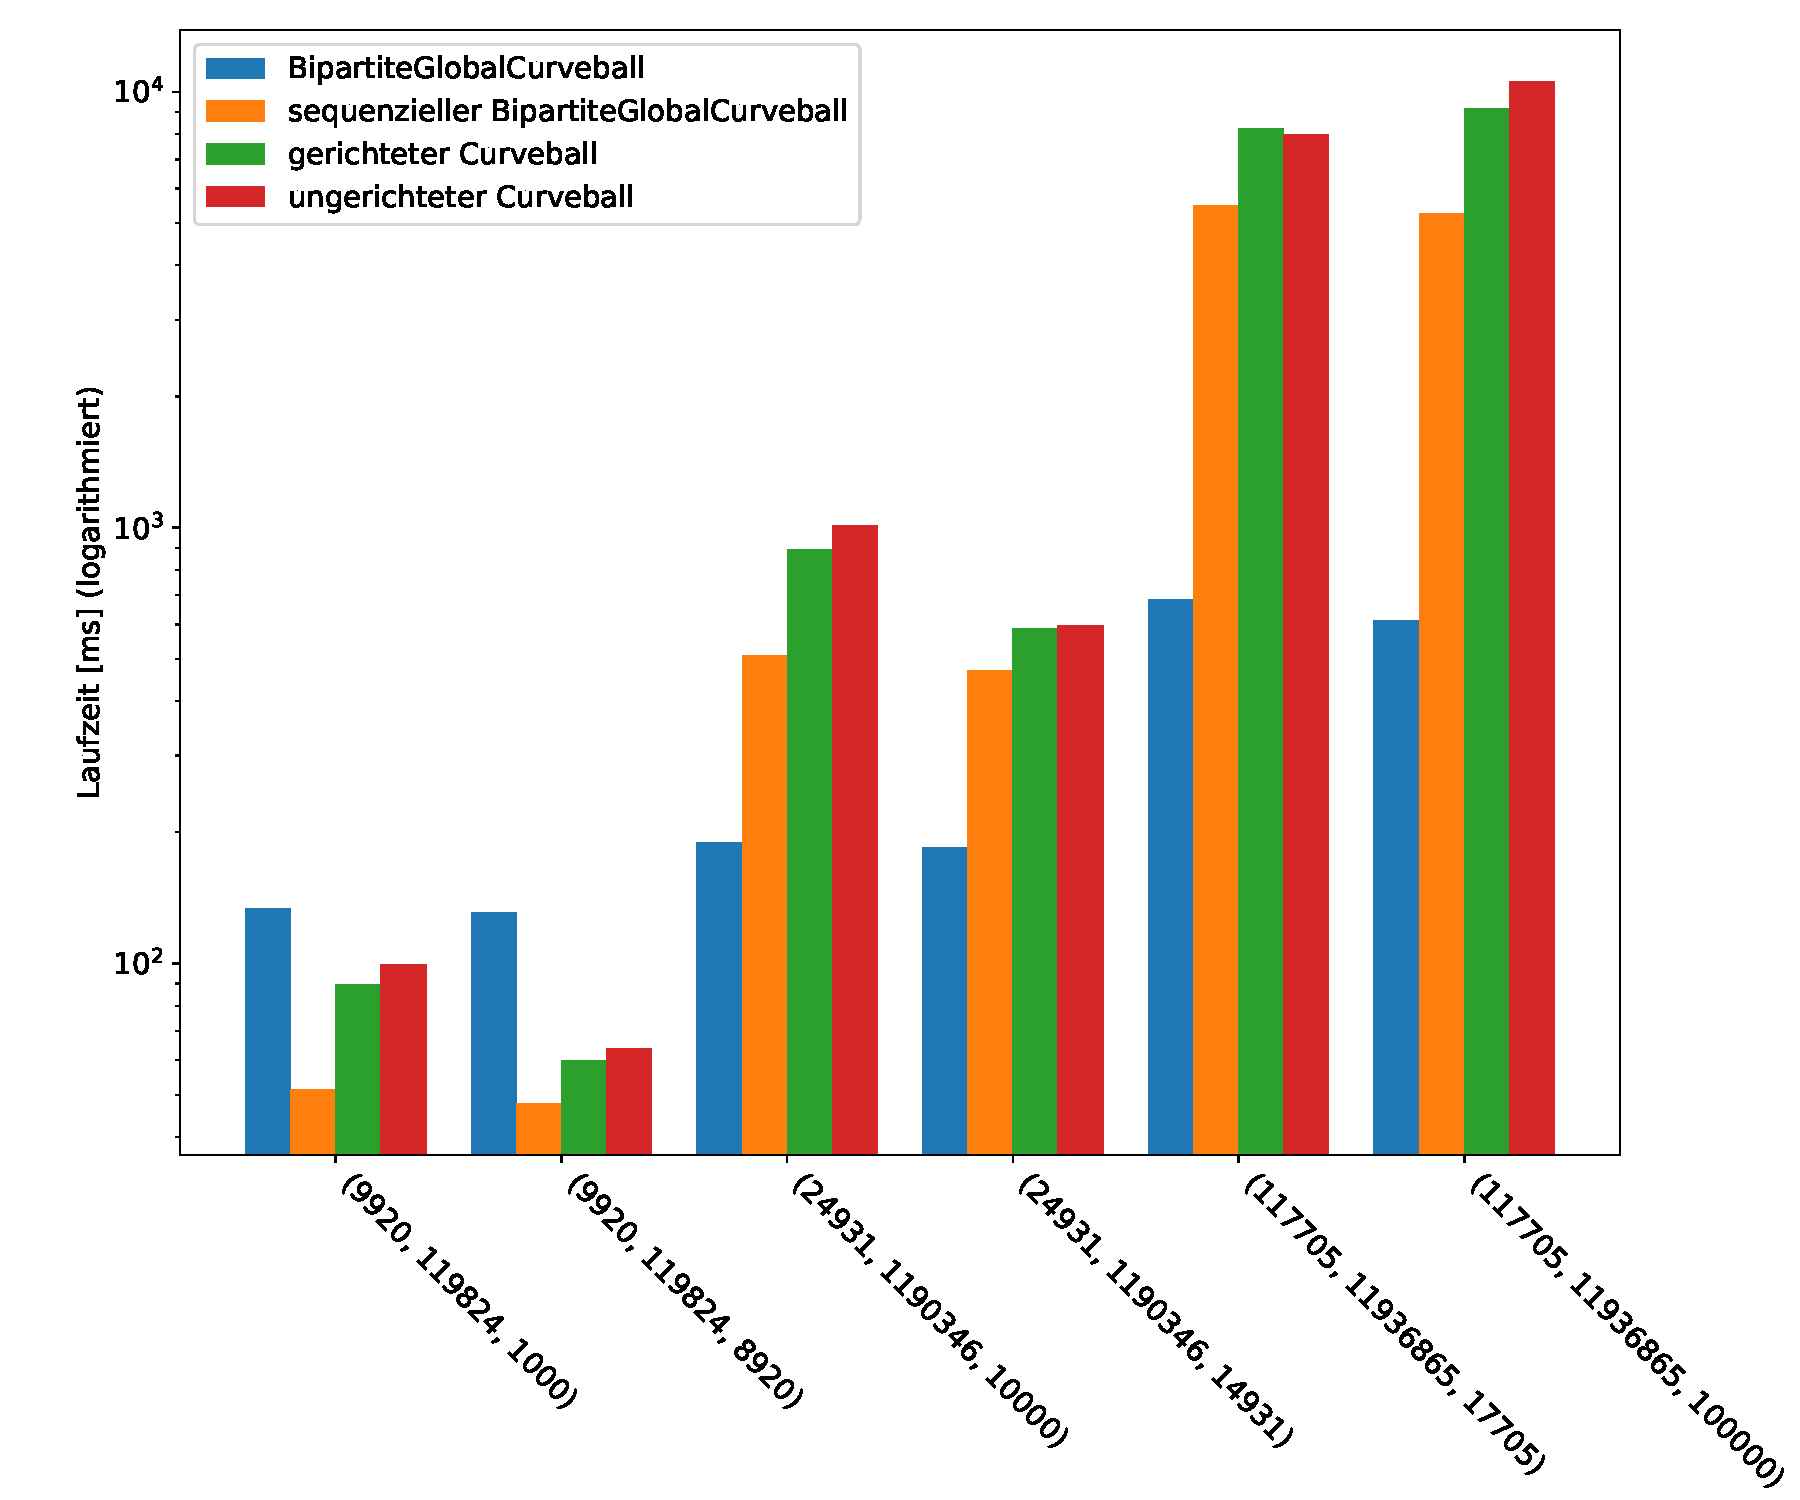
\includegraphics[width = 0.8\textwidth]{figures/speedup.pdf}
	\caption[Laufzeitvergleich von bipartitem \gc{} und einer abgeänderten Variante von \cb{}]{Laufzeitvergleich von bipartitem \gc{} und der abgeänderten Version des \cb{s}.{}
	Auf der horizontalen Achse sind die einzelnen Instanzen als Tripel aufgetragen.
Die erste Stelle steht dabei für die Knotenanzahl des Graphen, 
die zweite Stelle für die Anzahl an Kanten und die dritte für die Anzahl der Knoten aus 
der aktiven Partition.}
	\label{fig:speedup_komplett}
\end{figure}
